\chapter{Analysis}
\label{chapter:analysis}

In this chapter the scan algorithms are examined with regard to possible
reduction of the required memory bandwidth. This is done under the assumption
that \simdscan{}, \bwv{} and \bs{} operate at or close to the bandwidth
limitations of a modern processor. As such, \simdscan{} represents the upper
bound of memory bandwidth as \simdscan{} and \bwv{} use in-memory representations
of the same size, just in different layouts. \bs{} is comparable for all bit
cases evenly divisible by eight. As possible bandwidth reductions the early
pruning behavior of \bwv{} and \bs{} is analyzed and for all three approaches
the impact of write size reduction by scanning a column in fixed-size blocks
instead of doing a full column scan when evaluating a query over multiple
columns. This lowers the amount of temporary results materialized in memory.

\section{Early Pruning Probabilities}

If a scan algorithm is limited by the available memory bandwidth there is only
one way to improve its performance further, reducing the amount of memory
touched by it. As the input data for \bwv{} is already packed with no padding
the only way to reduce the number of bytes read during a scan without changing
the input data is aborting the scan of a given code word early. The
effectiveness of this approach relies on three factors:

\begin{itemize}
  \item the predicate,
  \item the selectivity,
  \item and the distribution of the input data.
\end{itemize}

Compared to \simdscan{}'s approach this adds a probabilistic dimension to the
runtime analysis of a scan. The simplest predicate to analyze is the equality
predicate. This predicate looks for values that are exactly the same as a
reference. In \bwv{} this is solved by looking at a value from the column and
the reference bit by bit, starting with the most significant, as shown for a
single value in algorithm~\ref{algo:equal}. In reality \bwv{} compares many
values in parallel.

\begin{algorithm}[h]
\begin{algorithmic}[1]
  \Procedure{IsEqual}{$a$, $b$}
    \For {$i \gets n-1$ to $0$}
      \If {$a_i \ne b_i$}
        \State \Return false
      \EndIf
    \EndFor
    \State \Return true
  \EndProcedure
\end{algorithmic}
\caption{Algorithm to check whether two bit vectors of size $n$ are equal}
\label{algo:equal}
\end{algorithm}

\paragraph{Establishing the Best and Worst Cases for Early Pruning}

It is now fairly simple to establish the best and worst cases for this scan. In
the best case all values $a$ from the column differ in the most significant bit
with the reference value $b$, for example $b$ is negative but all $a$s are
positive values. In this case only the most significant bit has to be read and
all other bits are ignored. The loop only executes a single iteration and the
selectivity is $0\,\%$. In the worst case all values $a$ are equal to $b$, in
this case the loop will always execute $n$ iterations and the selectivity is a
$100\,\%$. No memory reads can be skipped, early pruning is entirely defeated.
However, if the overhead of the pruning scan is low enough this worst case will
have the same performance characteristics as the \simdscan{}, it reads exactly
the same amount of data.

% TODO: reevaluate whether expected value is the right measure here

Now of course \bwv{} does not look at bits individually but will start by
reading a number of most significant bits at the same time and perform the
comparison in parallel. For example an implementation targeting the 256 bit
registers in Intel's AVX~2 instruction set extension will read bits from 256
values at the same time, perform the comparison and advance to the next 256 bits
of the same values. This however means that if at least one of those 256 values
is equal to the reference value the worst case is automatically triggered for
256 values. For uniformly distributed data the expected value for a selectivity
where early pruning still has an effect and not all bits must be read is as low
as $$E[S]=\frac{1}{256}\approx 0.4\,\%$$ In other words, the worst case can be
achieved by placing one equal value in every 256 values.

For \bs{} the worst case is always eight times better as fewer values are being
processed in parallel. For an AVX~2 implementation only 32 eight-bit slices are
compared at the same time, pushing the minimum selectivity needed for the worst
case up to $$E[S]=\frac{1}{32}\approx 3.1\,\%$$

\paragraph{Putting It on Real Hardware}

On current server-class hardware \bwv{} can easily hit memory bandwidth
limitations. This has an effect on the early pruning probabilities too as
memory is loaded in cache line-sized chunks. Only if an entire cache line can
be skipped a reduction in memory bandwidth (and thus scan performance) can be
achieved. On the tested Intel hardware a cache line consists of 512 bits,
meaning the theoretical worst case is off by a factor of two. For a uniform
distribution of equal values the worst case selectivity for \bwv{} becomes
$$E[S]=\frac{1}{512}\approx 0.2\,\%$$ as every cache line contains bits of 512
values. For \bs{} which only uses bytes and stores bits of 64 value per cache
line it goes down to $$E[S]=\frac{1}{64}\approx 1.6\,\%$$ As long as the cache
line size is larger than the register size, the register size has no effect on
the early pruning probability. As soon as the computation is fast enough so the
scan is only limited by memory bandwidth further increases or decreases of the
register size will not have any effect on scan performance.

\paragraph{Calculating the Early Pruning Probability For A Given Bit}

Now that we have established the worst and best cases we can look at the
average cases. For uniformly distributed data where any bit can be set with a
probability of $50\,\%$ the probability that a given value is equal with the
reference value up to bit $b$ is ${\left(\frac{1}{2}\right)}^b$,
so the full probability that we skip a cache line when reading bit $b$ is
$$P(b)={\left(1-{\left(\frac{1}{2}\right)}^b\right)}^{512}$$
for \bwv{}~\cite{BitWeaving} and
$$P(b)={\left(1-{\left(\frac{1}{2}\right)}^b\right)}^{64}$$
for \bs{}~\cite{ByteSlice}. Both rapidly approach $100\,\%$ for high bit widths,
with \bs{} having a huge advantage over \bwv{} at position eight and still being
better at position sixteen as seen in
figure~\ref{fig:earlypruningprobabilities}.

\begin{figure}[h] \center
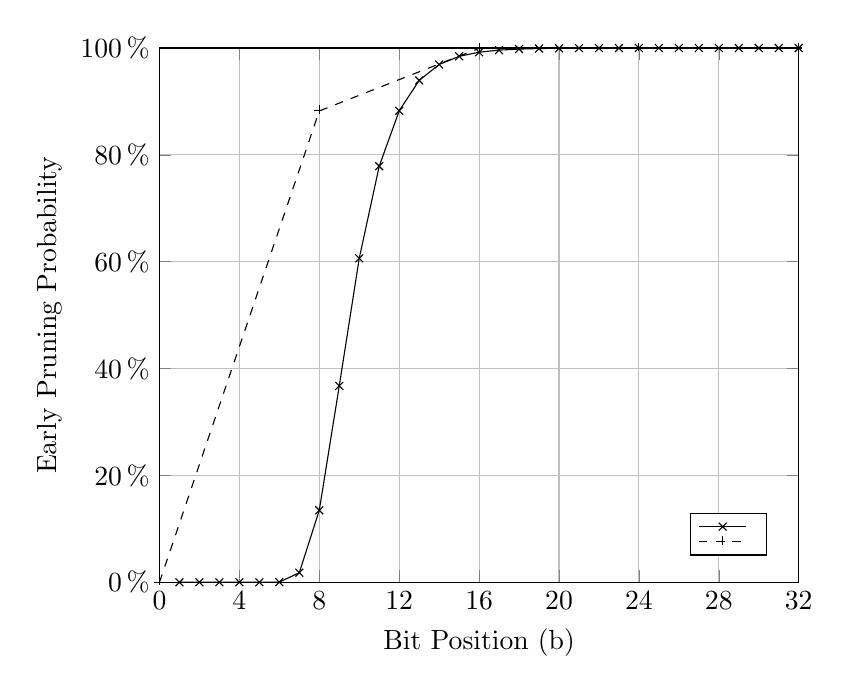
\begin{tikzpicture} \begin{axis}[
  grid,
  width=0.8*\textwidth,
  xlabel=Bit Position (b),
  ylabel=Early Pruning Probability,
  yticklabel=\pgfmathparse{100*\tick}\pgfmathprintnumber{\pgfmathresult}\,\%,
  xmin=0, xmax=32,
  ymin=0, ymax=1,
  legend entries={\bwv, \bs},
  legend style={at={(.95,.05)},anchor=south east},
  xtick={0,4,8,12,16,20,24,28,32}
]
\addplot+[black, mark=x, domain=1:32, samples=32] {(1-.5^x)^512};
\addplot+[black, mark=+, dashed, samples at={0,8,16,24,32}] {(1-.5^x)^32};
\end{axis}
\end{tikzpicture}
\caption{Early Pruning Probabilities for \bwv{} and \bs{}}
\label{fig:earlypruningprobabilities}
\end{figure}

For both \bwv{} and \bs{} there can be a significant hit due to branch
mispredictions in the early pruning code if pruning triggers irregularly. In the
range of bit widths between 1 and 32 bits the most mispredictions will occur for
code widths between 8 and 16 bits as the probabilities are not close to $0\,\%$
or $100\,\%$. This can severely impact the runtime of the scan.  To
reduce this effect \bwv{} partitions the bits into groups and only after a full
group has been processed the pruning branch is executed. \bs{} has an intrinsic
group size of eight so no additional handling is needed, but it is also less
flexible. This does not have an effect on early pruning probabilities but
reduces the amount of memory pruned away.

\paragraph{Worst and Best Cases for Other Predicates}

\begin{algorithm}[h]
\begin{algorithmic}[1]
  \Procedure{IsLess}{$a$, $b$}
    \For {$i \gets n-1$ to $0$}
      \If {$a_i \ne b_i$}
        \State \Return $a_i < b_i$
      \EndIf
    \EndFor
    \State \Return false
  \EndProcedure
\end{algorithmic}
\caption{Algorithm to check whether bit vector of size $n$ $a$ is less than $b$}
\label{algo:less}
\end{algorithm}

For the other predicates $<,\le,>,\ge$ and \textsc{between} the worst and best
cases are basically the same as for equality and inequality predicates, they are
triggered by exactly the same data.  However, there is no direct link between
the worst case and selectivity anymore. For $<,\le,>,\ge$ the worst case is hit
when all data is equal to the reference constant as seen in
algorithm~\ref{algo:less}. For \textsc{between} there is a slight difference as
both boundaries have to be taken into account as the computation is only aborted
when neither has a current bit equal to the value processed
(algorithm~\ref{algo:between}).

\begin{algorithm}[h]
\begin{algorithmic}[1]
  \Procedure{IsBetween}{$a$, $b$, $c$}
    \State isGreater $\gets$ false
    \State isLess $\gets$ false
    \For {$i \gets n-1$ to $0$}
      \State isGreater $\gets$ isGreater \textbf{or} $a_i > b_i$
      \State isLess $\gets$ isLess \textbf{or} $a_i < c_i$
      \If {$a_i \ne b_i$ \textbf{and} $a_i \ne c_i$}
        \State \Return isGreater \textbf{and} isLess
      \EndIf
    \EndFor
    \State \Return false
  \EndProcedure
\end{algorithmic}
\caption{Algorithm to check whether bit vector of size n $a$ is between $b$ and $c$}
\label{algo:between}
\end{algorithm}

\paragraph{Pruning Between Columns}

Another application of early pruning is discarding elements early when
evaluating a predicate over multiple columns. For example in
figure~\ref{fig:columnpruning} a conjunctive predicate over three columns is
evaluated, completely gray colored rows were skipped due to row the already being
discarded in the previous column. The regular \bwv{}-style early pruning is
also applied. This can be extremely effective for conjunctive predicates with
very low selectivity or disjunctive predicates with very high selectivity as
large parts of the later columns can be pruned away.  The order in which the
columns are scanned is now also important, a query optimizer could decide on the
evaluation order based on its selectivity information.

Intra-column pruning also applies to scan algorithms that do not generally
support early pruning, such as \simdscan{}.

\begin{figure}\center
\begin{tikzpicture}[node distance=4cm]
\tikzset{
table/.style={
  matrix of nodes,
  row sep=-\pgflinewidth,
  column sep=-\pgflinewidth,
  nodes={rectangle,draw=black,text width=1.25ex,align=center},
  text depth=0.25ex,
  text height=1ex
  },
}

\matrix[table] (mat1) {
 0 & |[fill=lightgray]| 0 & |[fill=gray]| 0 \\
 0 & 1 & |[fill=lightgray]| 0 \\
 0 & |[fill=lightgray]| 0 & |[fill=gray]| 1 \\
|[fill=lightgray]| 1 & |[fill=gray]| 0 & |[fill=gray]| 1 \\
};

\node[above of=mat1, node distance=1.5cm] {$A < 3$};
\draw[thick,->,right of=mat1] (-3,0) -- node[anchor=south] {and} (-1,0);

\matrix[table, right of=mat1] (mat2) {
 0 & 0 & |[fill=lightgray]| 1 \\
 0 & 0 & 0 \\
 0 & |[fill=lightgray]| 1 & |[fill=gray]| 1 \\
|[fill=gray]| 1 & |[fill=gray]| 0 & |[fill=gray]| 1 \\
};

\node[above of=mat2, node distance=1.5cm] {$B < 1$};
\draw[thick,->,right of=mat2] (1,0) -- node[anchor=south] {and} (3,0);

\matrix[table, right of=mat2] (mat3) {
|[fill=gray]| 1 & |[fill=gray]| 1 & |[fill=gray]| 1 \\
 1 & 1 & |[fill=lightgray]| 0 \\
|[fill=gray]| 0 & |[fill=gray]| 1 & |[fill=gray]| 1 \\
|[fill=gray]| 1 & |[fill=gray]| 0 & |[fill=gray]| 0 \\
};

\node[above of=mat3, node distance=1.5cm] {$C < 7$};
\end{tikzpicture}
\caption{Evaluation of the predicate $A < 3$ and $B < 1$ and $C < 7$ on three
columns}
\label{fig:columnpruning}
\end{figure}

\section{Block-Wise Scanning}

The output of a scan as performed by \bwv{} and \bs{} is a bit vector with one
bit for every value in the input. Depending on the result of the predicate the
bit is either set or not set. Traditionally a column is scanned in its entirety,
the result bit vector is written to memory and the scan proceeds to the next
column. This means that an extra bit per value has to be written to memory for
the intermediate results which is not needed for the end result. To reduce
bandwidth the columns are now partitioned into fixed-size blocks. After a block
is scanned, the bit vector is kept in cache and the algorithm proceeds scanning
the next column. This is repeated for all columns, the final result is written
and the scan advances to the next set of blocks.

The bus between the processor and main memory is not capable of full duplex
operation so any reduction in write bandwidth counts directly towards the total
bandwidth. The reduction is particularly significant for small bandwidths, for
example for a four-bit scan of two columns the total bandwidth would be ten
bits, eight read and two written. Block-wise scanning reduces this to nine
bits, a $10\,\%$ reduction. Figure~\ref{fig:blockwisesavings} shows reductions
for scans over four and sixteen columns, for simplicity all columns are of the
same bit width. The savings are calculated by dividing the saved bits by the
total bit bandwidth without block-wise scanning, $\frac{c-1}{c(b+1)}$ where $c$
is the number of columns and $b$ is the bit width.

\begin{figure}[h] \center
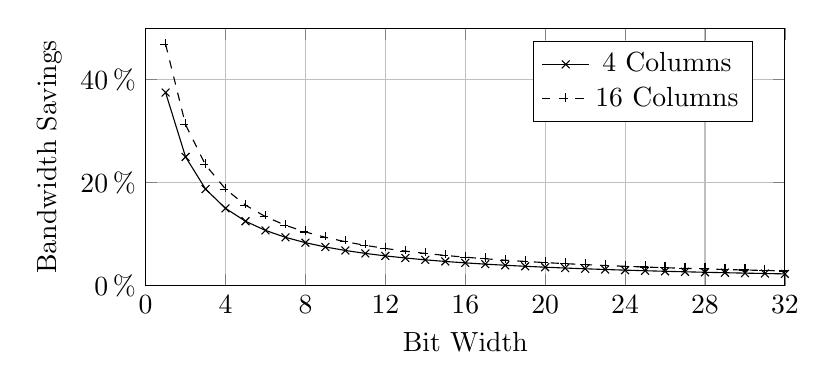
\begin{tikzpicture} \begin{axis}[
  grid,
  width=0.8*\textwidth,
  height=0.4*\textwidth,
  xlabel=Bit Width,
  ylabel=Bandwidth Savings,
  yticklabel=\pgfmathparse{100*\tick}\pgfmathprintnumber{\pgfmathresult}\,\%,
  xmin=0, xmax=32,
  ymin=0, ymax=.5,
  legend entries={4 Columns, 16 Columns},
  legend style={at={(0.95,0.95)},anchor=north east},
  xtick={0,4,8,12,16,20,24,28,32}
]
\addplot+[black, mark=x, domain=1:32, samples=32] {3/((x+1)*4)};
\addplot+[black, mark=+, dashed, domain=1:32, samples=32] {15/((x+1)*16)};
\end{axis}
\end{tikzpicture}
\caption{Potential bandwidth savings through block-wise scanning}
\label{fig:blockwisesavings}
\end{figure}

The potential downside for large column counts is that it can destroy the
regular consecutive access pattern of the memory. Modern processors are
optimized to recognize this pattern and pre-fetch following accesses. Since
this is the reason why column scans are fast a significant performance hit will
be seen if the pre-fetching stops working due to changed access patterns.

The block-wise technique works for all kinds of scan algorithms, including
\simdscan{}, \bwv{} and \bs{}.

Since \bwv{} with AVX~2 always processes 256 elements at a time it would be
reasonable to pick 256 as the block size and keep the intermediate values in
registers at all time. Since the \bwv{} implementation is limited by DRAM
bandwidth and intermediate values will stay in cache unless the block size is
very large this is unlikely to have a performance impact in comparison to other
sizes though.
